\documentclass[lualatex,ja=standard,a4paper,12pt]{bxjsarticle}
\usepackage{amsmath, amssymb, amsthm}
\usepackage{geometry}
\usepackage{xcolor}
\usepackage{tcolorbox}
\usepackage{booktabs}
\usepackage{array}
\usepackage{graphicx}

\geometry{margin=25mm}

\tcbuselibrary{theorems, skins, breakable}

\newtcolorbox{defbox}[1]{
  colback=blue!5, colframe=blue!60!black,
  fonttitle=\bfseries, title={#1}, arc=3pt, breakable
}
\newtcolorbox{thmbox}[1]{
  colback=green!5, colframe=green!50!black,
  fonttitle=\bfseries, title={#1}, arc=3pt, breakable
}
\newtcolorbox{pointbox}{
  colback=orange!8, colframe=orange!70!black,
  fonttitle=\bfseries, title={ポイント}, arc=3pt, breakable
}
\newtcolorbox{exbox}[1]{
  colback=gray!6, colframe=gray!50,
  fonttitle=\bfseries, title={例：#1}, arc=3pt, breakable
}
\newtcolorbox{warningbox}{
  colback=red!5, colframe=red!60!black,
  fonttitle=\bfseries, title={注意}, arc=3pt, breakable
}

\title{\textbf{ガンマ分布とカイ二乗分布} \\[4pt]
       {\normalsize 補足資料：パラメータの役割と両者の関係}}
\author{}
\date{}

\begin{document}
\maketitle
\thispagestyle{empty}

% ===========================
\section{ガンマ分布の定義}
% ===========================

\begin{defbox}{ガンマ分布（rate パラメータ表記）}
$y > 0$ に対して，
\[
  \mathrm{dgamma}(y;\, \alpha, \beta)
  = \frac{\beta^\alpha}{\Gamma(\alpha)}\, y^{\alpha - 1} e^{-\beta y},
  \qquad \alpha > 0,\; \beta > 0.
\]
$\alpha$ を\textbf{形状（shape）パラメータ}，
$\beta$ を\textbf{レート（rate）パラメータ}と呼ぶ．
$\Gamma(\alpha)$ はガンマ関数で，密度の積分を1にするための正規化定数
（$\alpha$ が正の整数なら $\Gamma(\alpha) = (\alpha-1)!$）．
\end{defbox}

\begin{warningbox}
ガンマ分布には\textbf{2通りのパラメータ表記}があり，文献により異なる：
\begin{itemize}
  \item \textbf{rate 表記}：$e^{-\beta y}$（Hoff はこちら．本資料もこちら）
  \item \textbf{scale 表記}：$e^{-y/\theta}$，ただし $\theta = 1/\beta$
        （R の \texttt{dgamma} のデフォルト第3引数や
        \texttt{scipy.stats.gamma} の \texttt{scale} はこちら）
\end{itemize}
ソフトウェアで計算するときは
「$\beta$ を渡すのか $1/\beta$ を渡すのか」を必ず確認すること．
\end{warningbox}

\medskip
\noindent 主な統計量：
\begin{center}
\renewcommand{\arraystretch}{1.6}
\begin{tabular}{lc}
\toprule
期待値 & $E[Y] = \dfrac{\alpha}{\beta}$ \\
分散 & $\mathrm{Var}[Y] = \dfrac{\alpha}{\beta^2}$ \\
最頻値（$\alpha \geq 1$ のとき） & $\dfrac{\alpha - 1}{\beta}$ \\
\bottomrule
\end{tabular}
\end{center}

% ===========================
\section{パラメータの役割：グラフで確認}
% ===========================

\begin{center}
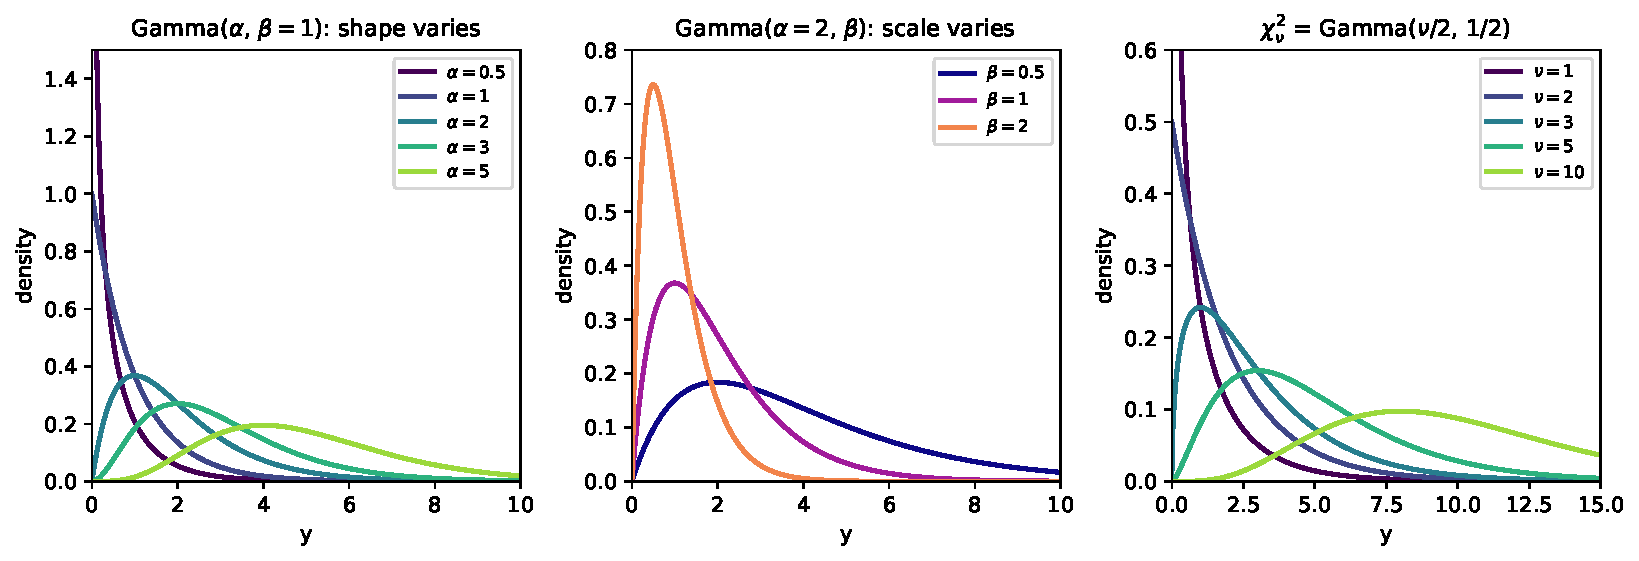
\includegraphics[width=\textwidth]{gamma_chi2_fig.pdf}
\end{center}

\subsection{$\alpha$（形状）：分布の「形」を決める}

第1パネルは $\beta = 1$ に固定して $\alpha$ を動かしたもの．
$\alpha$ の値によって形が\textbf{質的に}変わる：

\begin{itemize}
  \item $\boldsymbol{\alpha < 1}$：密度が $y \to 0$ で\textbf{発散}する
        （$y^{\alpha-1}$ の指数が負になるため）．
        原点近くに大量の確率が集まる．
  \item $\boldsymbol{\alpha = 1}$：$\mathrm{dgamma}(y; 1, \beta) = \beta e^{-\beta y}$，
        つまり\textbf{指数分布}に一致する．密度は $y=0$ で最大値 $\beta$ を取り単調減少．
  \item $\boldsymbol{\alpha > 1}$：密度は $0$ から立ち上がり，
        最頻値 $(\alpha-1)/\beta$ で山を作る\textbf{単峰型}になる．
  \item $\boldsymbol{\alpha}$ \textbf{が大きい}：
        山が対称に近づき，正規分布に似てくる
        （歪度は $2/\sqrt{\alpha} \to 0$）．
\end{itemize}

\subsection{$\beta$（レート）：分布の「ものさし」を決める}

第2パネルは $\alpha = 2$ に固定して $\beta$ を動かしたもの．
$\beta$ を変えても形は変わらず，
\textbf{横軸の縮尺だけ}が変わる．正確には
\[
  Y \sim \mathrm{Gamma}(\alpha, 1)
  \;\Longrightarrow\;
  \frac{Y}{\beta} \sim \mathrm{Gamma}(\alpha, \beta)
\]
という\textbf{尺度変換}の関係がある．
$\beta$ が大きいほど分布は原点側に圧縮される
（期待値 $\alpha/\beta$ が小さくなる）．

\begin{pointbox}
まとめ：\textbf{$\alpha$ が形，$\beta$ がスケール}．
より一般に，$Y \sim \mathrm{Gamma}(\alpha, \beta)$ で $c > 0$ なら
$cY \sim \mathrm{Gamma}(\alpha, \beta/c)$ が成り立つ．
この性質は次節でカイ二乗分布との関係を導くときに使う．
\end{pointbox}

\subsection*{その他の重要な性質：再生性}

独立に $Y_1 \sim \mathrm{Gamma}(\alpha_1, \beta)$，
$Y_2 \sim \mathrm{Gamma}(\alpha_2, \beta)$ ならば
\[
  Y_1 + Y_2 \sim \mathrm{Gamma}(\alpha_1 + \alpha_2, \beta).
\]
$\beta$ が共通なら，和を取ると $\alpha$ が足し算になる（\textbf{再生性}）．

% ===========================
\section{カイ二乗分布}
% ===========================

\begin{defbox}{カイ二乗分布}
$Z_1, \ldots, Z_\nu$ が i.i.d. $\mathrm{Normal}(0, 1)$ のとき，
\[
  Z_1^2 + Z_2^2 + \cdots + Z_\nu^2 \;\sim\; \chi^2_\nu
\]
と定義する．$\nu$ を\textbf{自由度}と呼ぶ．
つまり $\chi^2_\nu$ は「独立な標準正規変数 $\nu$ 個の2乗和の分布」．
\end{defbox}

\subsection{カイ二乗分布はガンマ分布の特殊ケース}

\begin{thmbox}{$\chi^2_\nu = \mathrm{Gamma}(\nu/2,\; 1/2)$}
自由度 $\nu$ のカイ二乗分布は，
形状 $\alpha = \nu/2$，レート $\beta = 1/2$ のガンマ分布に一致する．
密度で書けば
\[
  p(y) = \frac{(1/2)^{\nu/2}}{\Gamma(\nu/2)}\, y^{\nu/2 - 1} e^{-y/2},
  \qquad y > 0.
\]
\end{thmbox}

\noindent\textbf{確認の道筋：}
\begin{enumerate}
  \item $Z \sim \mathrm{Normal}(0,1)$ のとき $Z^2$ の密度を変数変換で求めると
        $\mathrm{Gamma}(1/2,\, 1/2)$ になる（これが $\chi^2_1$）．
  \item 独立なガンマ変数の和は再生性により $\alpha$ が足される：
        $Z_1^2 + \cdots + Z_\nu^2 \sim
         \mathrm{Gamma}(\underbrace{\tfrac12 + \cdots + \tfrac12}_{\nu \text{ 個}},\, \tfrac12)
         = \mathrm{Gamma}(\nu/2,\, 1/2)$．
\end{enumerate}

\subsection{Step 1 の証明：$Z^2 \sim \mathrm{Gamma}(1/2,\, 1/2)$}

$Y = Z^2$ とおき，$Y$ の密度を求める．

\begin{warningbox}
変換 $z \mapsto z^2$ は\textbf{1対1ではない}：
$Y = y$ に対応する $Z$ の値は $+\sqrt{y}$ と $-\sqrt{y}$ の\textbf{2つ}ある．
このため「逆関数を代入してヤコビアンを掛ける」だけの
1対1用の変数変換公式はそのまま使えない．
安全なのは，いったん累積分布関数（CDF）に戻ってから微分する方法である．
\end{warningbox}

\paragraph{CDF 経由の導出}
$y > 0$ に対して，$Y$ の CDF は
\[
  F_Y(y) = P(Z^2 \leq y)
         = P(-\sqrt{y} \leq Z \leq \sqrt{y})
         = \Phi(\sqrt{y}) - \Phi(-\sqrt{y})
         = 2\Phi(\sqrt{y}) - 1,
\]
ここで $\Phi$ は標準正規の CDF，最後の等号は標準正規の対称性
$\Phi(-x) = 1 - \Phi(x)$ による．
これを $y$ で微分すれば密度が得られる．
$\Phi' = \varphi$（標準正規密度）と合成関数の微分より
\[
  f_Y(y) = \frac{d}{dy}\left[2\Phi(\sqrt{y}) - 1\right]
         = 2\,\varphi(\sqrt{y}) \cdot \frac{1}{2\sqrt{y}}
         = \frac{\varphi(\sqrt{y})}{\sqrt{y}}.
\]
$\varphi(x) = \frac{1}{\sqrt{2\pi}} e^{-x^2/2}$ を代入すると
\[
  f_Y(y)
  = \frac{1}{\sqrt{2\pi}}\, y^{-1/2}\, e^{-y/2},
  \qquad y > 0.
\]

\paragraph{ガンマ密度との照合}
一方，$\mathrm{Gamma}(1/2,\, 1/2)$ の密度は定義より
\[
  \mathrm{dgamma}\!\left(y;\, \tfrac12, \tfrac12\right)
  = \frac{(1/2)^{1/2}}{\Gamma(1/2)}\, y^{1/2 - 1} e^{-y/2}
  = \frac{1}{\sqrt{2}\,\Gamma(1/2)}\, y^{-1/2} e^{-y/2}.
\]
$y$ への依存の仕方（$y^{-1/2} e^{-y/2}$）は完全に一致しているので，
あとは定数が一致すればよい．
ガンマ関数の有名な特殊値 $\Gamma(1/2) = \sqrt{\pi}$ を使うと
\[
  \frac{1}{\sqrt{2}\,\Gamma(1/2)}
  = \frac{1}{\sqrt{2}\cdot\sqrt{\pi}}
  = \frac{1}{\sqrt{2\pi}}
\]
となり，先ほどの $f_Y$ と完全に一致する．よって
\[
  Z^2 \sim \mathrm{Gamma}\!\left(\tfrac12,\, \tfrac12\right) = \chi^2_1.
  \qquad \blacksquare
\]

\begin{pointbox}
2つの補足：
\begin{itemize}
  \item 逆に見れば，「$f_Y$ は密度だから積分して1になる」ことと
        ガンマ密度の正規化定数を見比べることで
        $\Gamma(1/2) = \sqrt{\pi}$ が\textbf{証明できる}．
        これはガウス積分 $\int_{-\infty}^{\infty} e^{-x^2/2}\,dx = \sqrt{2\pi}$
        と同値な事実である．
  \item $\alpha = 1/2 < 1$ なので $\chi^2_1$ の密度は $y \to 0$ で発散する
        （図の第3パネル $\nu=1$ の曲線）．
        これは「$Z$ が0付近の値を取りやすい $\Rightarrow$ $Z^2$ は
        0のごく近くに確率が集中する」ことの現れである．
\end{itemize}
\end{pointbox}

\medskip
\noindent
第3パネルは $\nu = 1, 2, 3, 5, 10$ の $\chi^2_\nu$ 密度である．
ガンマ分布の $\alpha$ の役割がそのまま現れている：
\begin{itemize}
  \item $\nu = 1$（$\alpha = 1/2 < 1$）：原点で発散
  \item $\nu = 2$（$\alpha = 1$）：指数分布 $\mathrm{Exp}(1/2)$ に一致
  \item $\nu \geq 3$（$\alpha > 1$）：単峰型，$\nu$ が増えると右へ移動し対称に近づく
\end{itemize}
主な統計量はガンマ分布の公式に代入すればよい：
$E[\chi^2_\nu] = \dfrac{\nu/2}{1/2} = \nu$，
$\mathrm{Var}[\chi^2_\nu] = \dfrac{\nu/2}{(1/2)^2} = 2\nu$．

\subsection{統計学でカイ二乗分布が現れる場面}

\begin{exbox}{標本分散の標本分布（Hoff 5.6節との接続）}
$Y_1, \ldots, Y_n$ が i.i.d. $\mathrm{Normal}(\theta, \sigma^2)$ のとき，
\[
  \frac{(n-1)\,s^2}{\sigma^2} \;\sim\; \chi^2_{n-1}.
\]
これに尺度変換の性質（$cY \sim \mathrm{Gamma}(\alpha, \beta/c)$）を使うと
\[
  \frac{(n-1)s^2}{\sigma^2} \sim \mathrm{Gamma}\!\left(\frac{n-1}{2}, \frac{1}{2}\right)
  \;\Longrightarrow\;
  s^2 \sim \mathrm{Gamma}\!\left(\frac{n-1}{2},\; \frac{n-1}{2\sigma^2}\right)
\]
となり，Hoff 5.6節の式
$p(s^2 \mid \bar{y}, \theta, \sigma^2) = \mathrm{dgamma}(s^2, \frac{n-1}{2}, \frac{n-1}{2\sigma^2})$
が得られる．
自由度が $n$ でなく $n-1$ になる理由と導出は
5.6節ゼミ資料の付録を参照．
\end{exbox}

\medskip
\noindent このほかにも，カイ二乗分布は
\begin{itemize}
  \item 分割表の\textbf{カイ二乗検定}（ピアソンの適合度検定）の帰無分布
  \item \textbf{尤度比検定}の統計量の漸近分布（Wilks の定理）
  \item ベイズ統計では $\sigma^2$ の共役事前分布
        （逆ガンマ分布＝「ガンマ分布の逆数」の分布）の基礎
\end{itemize}
として頻繁に登場する．

% ===========================
\section{まとめ}
% ===========================

\begin{thmbox}{まとめ}
\begin{enumerate}
  \item ガンマ分布 $\mathrm{Gamma}(\alpha, \beta)$ は正の値を取る量の
        代表的な分布．\textbf{$\alpha$ が形}（発散／指数型／単峰型），
        \textbf{$\beta$ がスケール}を決める．
        期待値は $\alpha/\beta$，分散は $\alpha/\beta^2$．
  \item rate 表記と scale 表記の2流儀があるので，
        文献・ソフトウェア間の変換に注意（Hoff は rate 表記）．
  \item カイ二乗分布 $\chi^2_\nu$ は「独立な標準正規 $\nu$ 個の2乗和」であり，
        ガンマ分布の特殊ケース $\mathrm{Gamma}(\nu/2, 1/2)$ にほかならない．
  \item 正規データの標本分散の分布
        $(n-1)s^2/\sigma^2 \sim \chi^2_{n-1}$ を
        ガンマ分布の言葉に直したものが，Hoff 5.6節で使われる
        $s^2 \sim \mathrm{Gamma}\!\left(\frac{n-1}{2}, \frac{n-1}{2\sigma^2}\right)$ である．
\end{enumerate}
\end{thmbox}

\end{document}
